\chapter{Methodology}
\label{ch:methodology}

\section{Overview of the Development Pipeline}

The development of the proposed hybrid AI image detector proceeded through four major phases: (i) dataset construction and quality assurance; (ii) forensic feature engineering and Phase-1 feature selection; (iii) model architecture design, training, and hyperparameter optimisation; and (iv) inference pipeline development and web deployment. These phases are described in detail in the following sections. Figure~\ref{fig:workflow} illustrates the overall development pipeline.

\begin{figure}[H]
    \centering
    % NOTE: Place the workflow diagram image in the img/ folder as img/workflow.png
    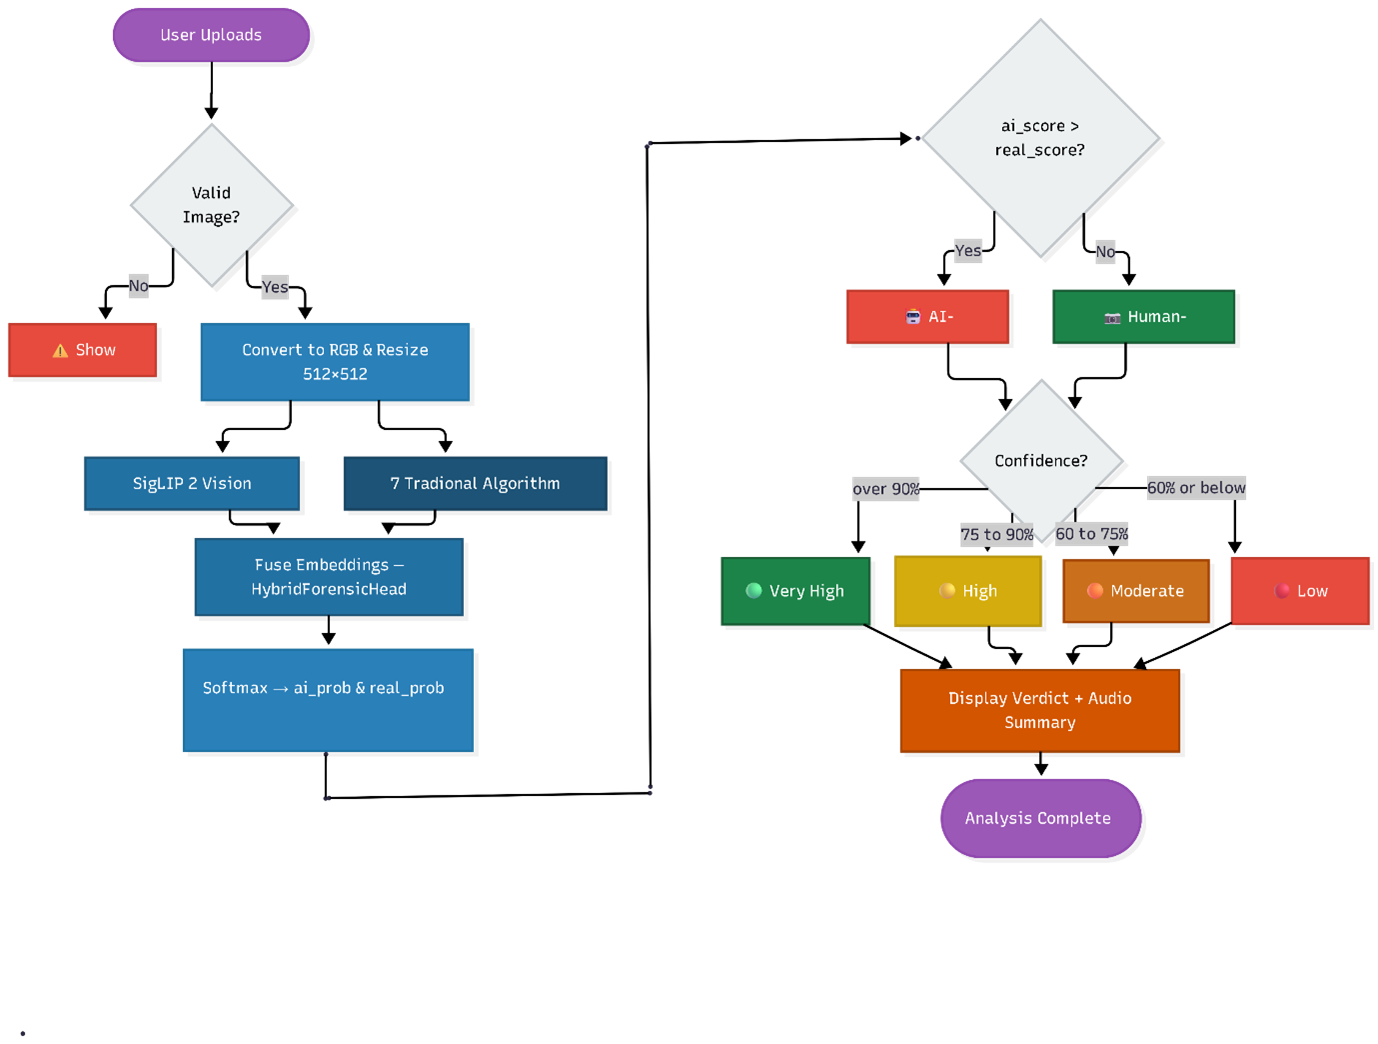
\includegraphics[width=0.9\textwidth]{img/workflow}
    \caption{Overall development pipeline for the hybrid AI image detector.}
    \label{fig:workflow}
\end{figure}

\section{Dataset Construction}

The dataset includes photos and AI-generated images from several platforms. This selection matches the variety found in real-world image distributions. We describe the collection methods and the partitioning scheme in the following sections.

\subsection{Data Collection Strategy}

The training data set was designed to reflect the nature and distribution of images that would be commonly found in real-world social media and internet settings, rather than the more typical academic benchmark data sets that have been employed in previous research. The data set was comprised of real-world images, totalling 4,400, gathered from various photography communities, including Reddit and Discord forums, and meticulously curated collections of high-quality images.

Images synthesized using AI, totalling 3,200, were gathered from the image galleries and export tools of five unique AI generative tools: Sora, an Open AI video/image model, Ideogram Explorer, Google Gemini image generation, ChatGPT DALL-E, and Leonardo AI, which employs variants of Stable Diffusion. The above approach was taken in order to ensure that the detector would be trained on images from both major paradigms of image generation: diffusion and multimodal generation, and to avoid overfitting against particular artifact patterns associated with a particular tool or tools.

\subsection{Dataset Splits}

The dataset consists of 7,600 images. These images are divided into 3 partitions called training, validation, and test. To divide this into 3 partitions, we used stratified sampling to preserve the class distribution across all splits. The 3 parts are split into 70\% for training (5,320 images), 15\% for validation (1,140 images), and 15\% for testing (1,132 images). Stratification preserved the original 58\% real and 42\% AI image ratio in each partition. The test set was held out from all model development decisions, including hyperparameter selection, and was used only for final performance reporting.

\begin{table}[htbp]
    \centering
    \caption{Dataset distribution across training, validation, and test splits.}
    \label{tab:dataset}
    \begin{tabular}{lccc}
        \toprule
        \textbf{Split} & \textbf{Total Images} & \textbf{Real} & \textbf{AI-Generated} \\
        \midrule
        Training        & 5,320 & 3,080 & 2,240 \\
        Validation      & 1,140 & 660   & 480   \\
        Test (Held-out) & 1,132 & 472   & 660   \\
        \midrule
        Total           & 7,592 & 4,212 & 3,380 \\
        \bottomrule
    \end{tabular}
\end{table}

\section{Forensic Feature Engineering}

A two-phase feature engineering process was adopted. In Phase~1, a broad set of candidate forensic signals was evaluated individually to identify those with meaningful discriminative power. In Phase~2, the seven selected features were integrated into the hybrid model as a jointly trained forensic branch. The following subsections describe the selection methodology and each individual feature extractor.

\subsection{Feature Selection Methodology}

Before the comprehensive model training process (Phase 2), a feature selection process (Phase 1) was carried out. A comprehensive set of candidate forensic features was extracted and evaluated over the entire set of 7,600 images using the Area Under the Receiver Operating Characteristic Curve (AUC-ROC) as the primary measure of discriminative power. Each feature was tested individually using a simple logistic regression classifier trained on that feature in isolation. Seven features with individual AUC of at least 0.61 were selected for the hybrid model training process. Table~\ref{tab:features} lists the selected features and their Phase-1 AUC scores.

\begin{table}[H]
    \centering
    \small
    \caption{Selected forensic features with Phase-1 individual AUC scores.}
    \label{tab:features}
    \begin{tabular}{c p{3cm} p{4cm} c p{3.8cm}}
        \toprule
        \textbf{No.} & \textbf{Feature Name} & \textbf{What It Measures} & \textbf{AUC} & \textbf{Why It Helps} \\
        \midrule
        1 & LBP Entropy           & Texture randomness across pixels          & 0.79 & AI images have unnaturally uniform or over-random texture patterns \\
        2 & DCT Blocking          & Frequency regularity in $8\times8$ blocks & 0.69 & AI images violate natural frequency distributions (Benford's Law) \\
        3 & Gradient Co-occ.      & Edge structure and complexity             & 0.68 & AI images have smoother, less varied gradient transitions \\
        4 & Haar Wavelet Energy   & Diagonal detail energy at multi-scale     & 0.66 & AI images lack fine diagonal detail compared to real photographs \\
        5 & FFT Power Slope       & High-to-low frequency energy ratio        & 0.64 & AI images cluster around $-2.5$ slope with unusual consistency \\
        6 & Bayer Noise Pattern   & Camera sensor inter-channel correlation   & 0.63 & Real cameras leave unique noise fingerprints absent in AI images \\
        7 & Edge Sharpness Grid   & Sharpness across 9 spatial zones          & 0.61 & AI images show unnatural centre-vs-periphery sharpness ratios \\
        \bottomrule
    \end{tabular}
\end{table}

\subsection{Local Binary Pattern (LBP) Entropy}

\begin{figure}[htbp]
    \centering
    % NOTE: Place the LBP visualisation in img/lbp.png
    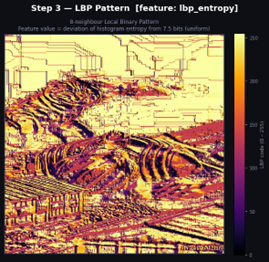
\includegraphics[width=0.45\textwidth]{img/lbp}
    \caption{LBP entropy feature map visualisation on an AI-generated image.}
    \label{fig:lbp}
\end{figure}

The Local Binary Pattern (LBP) operator characterises the micro-texture structure of an image by comparing each pixel's intensity with its eight immediate neighbours. For each pixel, a binary code is generated: 1 if a neighbour's intensity is greater than or equal to the middle pixel, or 0 if not. The image is then processed into a 256-bin histogram, and the Shannon entropy of this histogram is used as the forensic signal:
\begin{equation}
    H = -\sum_{i=0}^{255} p_i \log_2 p_i
\end{equation}
Entropy reaches a theoretical maximum of about 7.5 bits when the distribution is perfectly uniform across all 256 patterns. This value is very close to what real photographs have, which have a mix of sharp edges, smooth gradients, and fine sensor noise. AI-generated images, which optimize for global aesthetic coherence instead of micro-texture physical realism, create LBP distributions that are consistently different. The feature score is given by the absolute difference from this maximum value scaled to $[0, 1]$ via a sigmoid. 

\subsection{DCT Blocking (Benford's Law Deviation)}

\begin{figure}[htbp]
    \centering
    % NOTE: Place the DCT visualisation in img/dct.png
    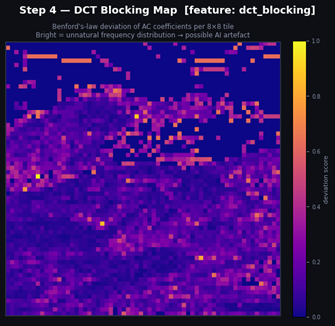
\includegraphics[width=0.5\textwidth]{img/dct}
    \caption{DCT Benford's Law deviation visualisation on an AI-generated image.}
    \label{fig:dct}
\end{figure}

The Discrete Cosine Transform (DCT) splits an image into $8 \times 8$ pixel blocks. It then turns these blocks into cosine frequency parts. Because cameras use the JPEG standard to handle photos this way, leaving a characteristic statistical fingerprint in the AC coefficients. In particular, the leading digits of these coefficients in real photographs follow Benford’s Law, which is the empirical regularity that smaller leading digits (1, 2, 3) are more common in natural numerical data than larger ones (7, 8, 9). AI-generated images, synthesised by neural networks that do not replicate the physical optics and compression pipeline of a real camera, produce DCT coefficient distributions that deviate from Benford's Law in measurable ways. The feature is computed as the chi-square deviation between the observed first-digit distribution and the Benford prediction, estimated from up to 400 randomly sampled $8 \times 8$ tiles.

\subsection{Gradient Co-occurrence Entropy}

\begin{figure}[htbp]
    \centering
    % NOTE: Place the gradient co-occurrence visualisation in img/gradient.png
    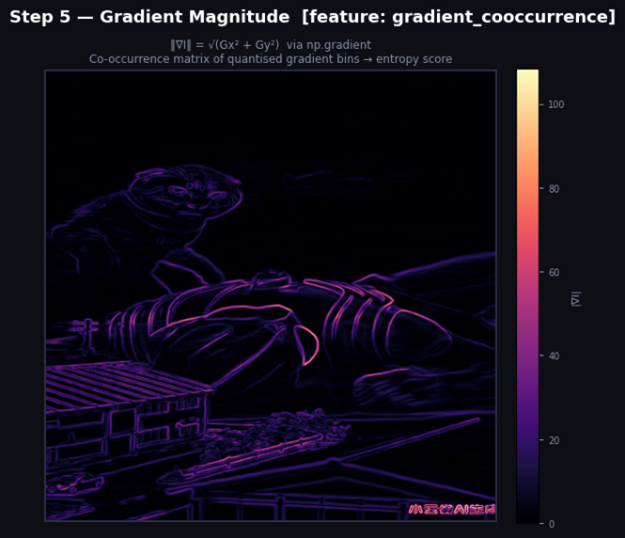
\includegraphics[width=0.48\textwidth]{img/gradient}
    \caption{Gradient co-occurrence entropy feature visualisation on an AI-generated image.}
    \label{fig:gradient}
\end{figure}

Edges in real photographs arise from physical boundaries between surfaces, changes in illumination, and depth transitions---processes that produce statistically complex, difficult-to-predict sequences of edge strengths. AI generators tend to produce edges that are either overly smooth and uniform or exhibit unnatural repetitive patterns. The gradient co-occurrence feature captures this by computing the gradient magnitude at every pixel, quantising these magnitudes into 32 bins, and building a $32 \times 32$ co-occurrence matrix that records the frequency of every pair of consecutive horizontal gradient magnitudes. The Shannon entropy of this co-occurrence matrix is used as the feature signal.

\subsection{Haar Wavelet Energy}

The Haar Wavelet Transform decomposes an image into four sub-bands at each pyramid level: a low-frequency approximation (LL), horizontal detail (LH), vertical detail (HL), and diagonal detail (HH). The HH sub-band captures edges and fine details oriented diagonally---a pattern that occurs naturally in real-world surfaces, camera optics, and noise, but is systematically suppressed in AI-generated images, which tend to produce locally over-smooth synthetic textures. The feature is computed as the ratio of HH sub-band energy to total detail energy (HH + LH + HL), averaged across three levels of a wavelet pyramid:
\begin{equation}
    E_{HH} = \frac{1}{3} \sum_{l=1}^{3} \frac{\|W_{HH}^{(l)}\|^2}{\|W_{HH}^{(l)}\|^2 + \|W_{LH}^{(l)}\|^2 + \|W_{HL}^{(l)}\|^2}
\end{equation}

\begin{figure}[H]
    \centering
    % NOTE: Place the Haar wavelet visualisation in img/haar.png
    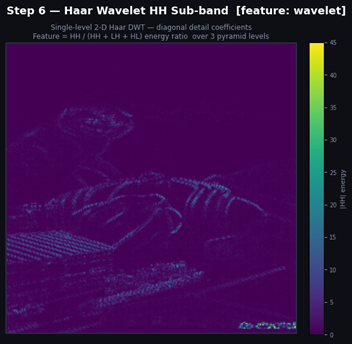
\includegraphics[width=0.55\textwidth]{img/haar}
    \caption{Haar wavelet diagonal sub-band energy visualisation on an AI-generated image.}
    \label{fig:haar}
\end{figure}

\subsection{FFT Power Slope}

\begin{figure}[htbp]
    \centering
    % NOTE: Place the FFT power slope visualisation in img/fft.png
    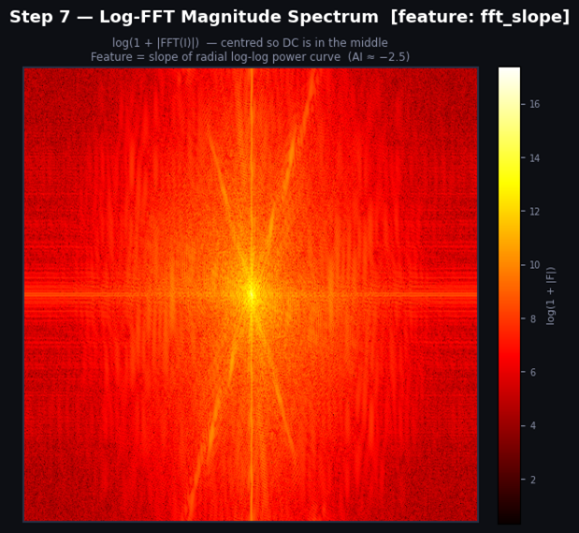
\includegraphics[width=0.48\textwidth]{img/fft}
    \caption{FFT power spectrum slope visualisation on an AI-generated image.}
    \label{fig:fft}
\end{figure}

The Fast Fourier Transform of a natural photograph, when analysed in log-log frequency space, follows a power-law relationship characterised by a slope of approximately $-2$ to $-3$: high-frequency components (fine details) are consistently less energetic than low-frequency components (large-scale structures). AI-generated images, particularly those from diffusion models and GANs, cluster unusually tightly around a slope of $-2.5$ with less variance than natural photographs, and sometimes show systematic deviations due to the frequency biases introduced by their decoder architectures. The feature is computed as:
\begin{equation}
    s = \left| \hat{\beta} - (-2.5) \right|
\end{equation}
where $\hat{\beta}$ is the fitted radial log-log slope, normalised and passed through a sigmoid function.

\subsection{Bayer Noise Pattern}

\begin{figure}[htbp]
    \centering
    % NOTE: Place the Bayer noise visualisation in img/bayer.png
    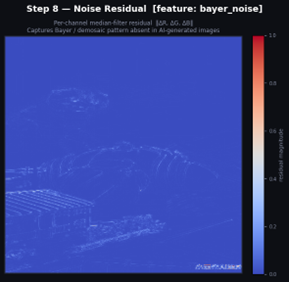
\includegraphics[width=0.48\textwidth]{img/bayer}
    \caption{Bayer noise inter-channel correlation visualisation on an AI-generated image.}
    \label{fig:bayer}
\end{figure}

Every digital camera sensor uses a Bayer colour filter array---a mosaic of alternating red, green, and blue photosensors. Because each physical pixel captures only one colour channel, a demosaicing algorithm must interpolate the other two channels from neighbouring pixels. This interpolation process introduces characteristic correlations between the red, green, and blue noise channels that serve as a unique physical fingerprint of real camera hardware. AI generators synthesise all three colour channels simultaneously and directly from learned distributions, so these inter-channel noise correlations are absent. The feature is extracted by applying a $3 \times 3$ median filter to each colour channel independently (to isolate the noise residual) and computing a weighted combination of the cross-channel spatial autocorrelation and cross-correlation metrics.

\subsection{Edge Sharpness Grid}

\begin{figure}[htbp]
    \centering
    % NOTE: Place the edge sharpness visualisation in img/edge.png
    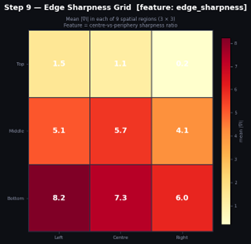
\includegraphics[width=0.45\textwidth]{img/edge}
    \caption{Edge sharpness grid visualisation on an AI-generated image.}
    \label{fig:edge}
\end{figure}

The optical characteristics of a camera lens---including depth of field, lens sharpness fall-off, and bokeh---create a characteristic spatial distribution of sharpness across a photograph. AI generators tend to produce images with either uniform sharpness across the entire frame, or synthetic depth-of-field effects that do not match the optical physics of any real lens. The feature divides the image into a $3 \times 3$ spatial grid of nine regions and measures the mean gradient magnitude (a proxy for local sharpness) in each region, producing a 9-dimensional sharpness distribution vector summarised into a scalar score reflecting the centre-vs-periphery sharpness ratio.

\section{Model Architecture}

The proposed architecture consists of three interconnected components: a SigLIP~2 vision backbone adapted for forensic classification, a dedicated MLP that embeds the traditional forensic feature vector, and a hybrid classification head that fuses both signal streams. Each component is described in detail below.

\subsection{SigLIP 2 Vision Backbone}

This system is built on SigLIP 2 \cite{tschannen2025siglip2}. We used the specific version from Hugging Face (\texttt{Ateeqq/ai-vs-human-image-detector}), which is already set up to tell the difference between real photos and AI-generated images. The text encoder and cross-modal projection components are surgically removed, leaving only the image encoder---a Vision Transformer (ViT) architecture with a patch size of 16 pixels and 1,024-dimensional patch embeddings. Retaining only the image encoder reduces the model's parameter count and memory footprint substantially while preserving the rich visual representations learned during the image-text alignment pre-training phase.

The position embeddings of the resulting vision encoder were originally pre-trained at a resolution of $224 \times 224$ pixels, corresponding to a $14 \times 14$ grid of 196 patches. To operate at $512 \times 512$ pixels, which preserves forensically important fine-grained details, the position embedding matrix is bicubically interpolated from the original $14 \times 14$ grid to a $32 \times 32$ grid of 1,024 patches. This interpolation is applied once before training and the new position embedding weights are treated as trainable parameters, allowing them to adapt to the forensic classification task during the subsequent fine-tuning phase. The image encoder thus accepts images of size $512 \times 512 \times 3$ and produces an output embedding of dimension 1,024.

\subsection{Traditional Forensic Feature MLP}

The seven-dimensional forensic feature vector extracted from each image is processed by a dedicated Feature MLP comprising three fully connected layers with the following structure:
\begin{itemize}
    \item Input layer: $7 \rightarrow 64$ with LayerNorm and GELU activation
    \item Intermediate layer: $64 \rightarrow 128$ with LayerNorm and GELU activation
    \item Output layer: $128 \rightarrow 128$
\end{itemize}
Dropout regularisation is applied after each non-linear activation. This MLP learns to embed the raw forensic feature scores into a 128-dimensional learned representation, allowing the model to discover non-linear combinations and interactions among the seven features that are more discriminative than the individual scores alone.

\subsection{Hybrid Classification Head with SE-Attention}

The 1,024-dimensional backbone embedding and the 128-dimensional forensic feature embedding are concatenated to produce a 1,152-dimensional fused representation. This fused vector is then processed by the Hybrid Forensic Head, a three-layer classification network:

\begin{itemize}
    \item \textbf{Layer 1:} Linear($1152 \rightarrow 1024$), BatchNorm1d, GELU activation, 40\% Dropout.
    \item \textbf{Attention:} SE-style ArtifactAttention module --- a squeeze-and-excitation network
    that computes a channel-wise attention weight vector from the 1,024-dimensional representation
    through a bottleneck MLP ($1024 \rightarrow 256 \rightarrow 1024$) with Sigmoid activation,
    then multiplies these weights element-wise into the representation.
    \item \textbf{Layer 2:} Linear($1024 \rightarrow 512$), BatchNorm1d, GELU activation, 30\% Dropout.
    \item \textbf{Layer 3 (Output):} Linear($512 \rightarrow 2$), producing raw logits for the two classes.
\end{itemize}

The SE style attention mechanism is the architectural innovation that distinguishes this head from regular classifiers. The attention module performs an implicit feature selection operation that enhances the most informative features for AI artifact detection while down-weighting irrelevant or noisy features.

\section{Training Strategy}

The model was trained using a carefully designed strategy that accounts for the heterogeneous nature of the hybrid architecture, balancing the pre-trained backbone against the randomly initialised classification components. The following subsections detail the hardware setup, the freeze-unfreeze schedule, the loss formulation, and the complete training algorithm.

\subsection{Training Setup}

Training was performed on Kaggle Notebooks using $2 \times$ T4 GPUs with 16 GB VRAM each. The model was trained for a maximum of 25 epochs with early stopping based on validation AUC, with a patience of 3 epochs. The effective batch size was 32 (8 per device $\times$ 2 GPUs $\times$ 2 gradient accumulation steps). Input images were resized to $512 \times 512$ during training using a smart adaptive resize strategy: images larger than $1024 \times 1024$ were first downsampled to $1024 \times 1024$ using LANCZOS anti-aliasing before the final bicubic resize to $512 \times 512$, to avoid aliasing artefacts in the forensic features. Training augmentations were restricted to forensically-safe operations: random JPEG compression (quality 70--98, applied with probability 0.4), quality balancing (probability 0.25), and random resized crop.

\subsection{Backbone Freeze-Unfreeze Schedule}

To prevent the rich SigLIP 2 representations from being immediately distorted by gradient updates from the randomly initialised classification head, the backbone was frozen during the first two training epochs. During this phase, only the Feature MLP and Hybrid Head parameters were updated, allowing the classification components to develop reasonable initial weights. From epoch 3 onwards, the backbone was unfrozen and all parameters were jointly optimised with a differential learning rate: a base learning rate of $2 \times 10^{-5}$ for the Feature MLP and Head, and a $10\times$ reduced learning rate ($2 \times 10^{-6}$) for the backbone parameters to prevent catastrophic forgetting.

\subsection{Loss Function and Class Weighting}

The training objective was class-weighted cross-entropy loss with label smoothing ($\varepsilon = 0.05$). Class weights were computed inversely proportional to class frequency in the training split: the AI class (3,200 images, 42.1\%) received a weight of 1.19, and the real class (4,400 images, 57.9\%) received a weight of 0.87. The loss function is defined as:
\begin{equation}
    \mathcal{L}(\hat{y}, y) = -\sum_{c} w_c \cdot \left[(1-\varepsilon) y_c + \frac{\varepsilon}{K}\right] \cdot \log(\hat{y}_c)
\end{equation}
where $K = 2$ classes, $w_c$ is the class weight, and $\varepsilon$ is the label smoothing factor. The AdamW optimiser was used with a cosine annealing learning rate schedule and a linear warmup phase covering the first 10\% of training steps.

\subsection{Formal Training Algorithm}

Algorithm~\ref{alg:training} presents the complete training pipeline.

\renewcommand{\arraystretch}{1.3}
\begin{longtable}{|p{0.92\textwidth}|}
\caption{Algorithm 4.1: Hybrid AI-Generated Image Detector Forensic Training Pipeline.}
\label{alg:training} \\
\hline
\small
\textbf{Input:} Image dataset $D = \{(x_i, y_i)\}$ where $x_i \in \mathbb{R}^{3 \times 512 \times 512}$, $y_i \in \{0=\text{AI}, 1=\text{Human}\}$; pre-computed Phase-1 features CSV with 7 forensic signals per image; fine-tuned SigLIP backbone. \\
\textbf{Output:} Fine-tuned hybrid classifier $f_\theta$; evaluation metrics \{Accuracy, F1, Precision, Recall, AUC-ROC, FPR, FNR\} \\
\hline
\endfirsthead
\hline
\multicolumn{1}{|c|}{\small\itshape (Algorithm 4.1 continued)} \\
\hline
\endhead
\hline
\endfoot
\hline
\endlastfoot
\small
\textbf{Step 1: Hardware Initialisation} \\
\quad a. Detect available CUDA devices; abort if no GPU found. \\
\quad b. Set DEVICE = ``cuda''; configure DataLoader with fp16=True. \\
\quad c. Effective batch size = BATCH\_PER\_GPU $\times$ $N_{GPU}$ $\times$ GRAD\_ACCUM = $8 \times N_{GPU} \times 4$. \\
\hline
\small\textbf{Step 2: Dataset Loading \& Class-Weight Computation} \\
\quad a. Recursively scan AI folder (label=0) and Real folder (label=1). \\
\quad b. Compute inverse-frequency class weights: $w_{AI} = N / (2 N_{AI})$; $w_{real} = N / (2 N_{real})$. \\
\quad c. Stratified 3-way split: Train 70\% $|$ Val 15\% $|$ Test 15\%; random seed = 42. \\
\hline
\small\textbf{Step 3: Phase-1 Feature Loading \& Scaling} \\
\quad a. Load pre-computed features.csv; verify all 7 feature columns exist. \\
\quad b. Apply sign inversion where needed; replace NaN with 0.5; clip all values to $[0, 1]$. \\
\quad c. Fit StandardScaler on full feature matrix; store in path $\rightarrow$ vector lookup table. \\
\hline
\small\textbf{Step 4: Model Architecture} \\
\quad a. Load SigLIP backbone; resize position embeddings from $14 \times 14$ to $32 \times 32$ via bicubic interpolation. \\
\quad b. Attach FeatureMLP: $7 \rightarrow 64 \rightarrow 128 \rightarrow 128$ with LayerNorm and GELU. \\
\quad c. Attach HybridForensicHead: $(d_{b}+128) \rightarrow 1024 \rightarrow$ SE-Attention $\rightarrow 512 \rightarrow 2$. \\
\hline
\small\textbf{Step 5: Training Loop (epochs $e = 1 \ldots 25$)} \\
\quad a. Freeze backbone for first 3 epochs; train only FeatureMLP and HybridHead. \\
\quad b. At epoch 3: unfreeze backbone for full joint fine-tuning. \\
\quad c. Forward: backbone $\rightarrow$ img\_emb; FeatureMLP $\rightarrow$ feat\_emb; concatenate $\rightarrow$ HybridHead $\rightarrow$ logits. \\
\quad d. Compute weighted cross-entropy with label smoothing $\varepsilon = 0.05$. \\
\quad e. Accumulate gradients for 4 steps; fp16 mixed precision. \\
\quad f. Save checkpoint if F1 improves; early stop if no improvement for 5 epochs. \\
\hline
\small\textbf{Step 6: Evaluation} \\
\quad a. Run inference on held-out test set (15\%) with no augmentation. \\
\quad b. Compute: Accuracy, Precision, Recall, F1, AUC-ROC, FPR, FNR. \\
\end{longtable}
\renewcommand{\arraystretch}{1}

\section{Inference Pipeline}

The inference pipeline was written in Python with PyTorch and Gradio for web interface deployment on Hugging Face Spaces. For each input image, the pipeline performs the following steps:

\begin{enumerate}
    \item \textbf{Image loading and validation:} Pillow loads the input image with truncated image handling enabled. The image is converted to RGB if not already in that format.
    \item \textbf{Adaptive resizing:} The image is resized to $512 \times 512$ using the adaptive resize strategy described in Section~4.5.1, with step-down only when the image exceeds $1024 \times 1024$ pixels.
    \item \textbf{Forensic feature extraction:} The seven forensic features are computed from the full-resolution resized image. The raw feature values are normalised using the StandardScaler statistics computed from the training set and stored in the model checkpoint.
    \item \textbf{Backbone inference:} The resized image is processed by the SigLIP 2 image processor (normalisation to ImageNet statistics) and passed through the backbone. The 1,024-dimensional embedding is extracted from the hidden states of the final transformer layer.
    \item \textbf{Fusion and classification:} The backbone embedding and the normalised forensic feature embedding are concatenated and passed through the Hybrid Forensic Head to produce class logits.
    \item \textbf{Output:} The softmax probabilities over the two classes are returned, along with the individual forensic feature scores for explainability. The total end-to-end latency measured on CPU hardware at Hugging Face Spaces is 142.4 milliseconds.
\end{enumerate}

\section{Tools and Technologies}

\begin{table}[htbp]
    \centering
    \caption{Tools and technologies used in development.}
    \label{tab:tools}
    \begin{tabular}{p{4.5cm} c p{6.5cm}}
        \toprule
        \textbf{Tool / Library} & \textbf{Version} & \textbf{Purpose} \\
        \midrule
        Python                    & 3.10         & Primary programming language \\
        PyTorch                   & 2.3          & Neural network implementation and training \\
        HuggingFace Transformers  & 4.41         & SigLIP 2 model loading and processing \\
        HuggingFace Datasets      & 2.19         & Dataset management and streaming \\
        NumPy / SciPy             & 1.26 / 1.13  & Forensic feature computation \\
        PyWavelets                & 1.6          & Haar Wavelet Transform implementation \\
        Pillow (PIL)              & 10.3         & Image loading and preprocessing \\
        Scikit-learn              & 1.5          & StandardScaler, metrics computation \\
        Gradio                    & 4.x          & Web inference interface (Hugging Face Spaces) \\
        Kaggle Notebooks          & N/A          & Training environment (dual T4 GPUs) \\
        \bottomrule
    \end{tabular}
\end{table}
